\documentclass{article}

\usepackage[utf8]{inputenc}
\usepackage[portuguese]{babel}
\usepackage{blindtext}
\usepackage{graphicx}
\usepackage{amsmath}
\usepackage{float}
\usepackage{caption}
\usepackage[compact]{titlesec}
\usepackage{multicol}
\usepackage[a4paper, total={7.5in, 10in}]{geometry}
\usepackage[font=scriptsize,labelfont=bf]{caption}
\usepackage{listings}
\usepackage{color}
 
\definecolor{codegreen}{rgb}{0,0.6,0}
\definecolor{codegray}{rgb}{0.5,0.5,0.5}
\definecolor{codepurple}{rgb}{0.58,0,0.82}
\definecolor{backcolour}{rgb}{0.95,0.95,0.92}
 
\lstdefinestyle{mystyle}{
    backgroundcolor=\color{backcolour},   
    commentstyle=\color{codegreen},
    keywordstyle=\color{magenta},
    numberstyle=\tiny\color{codegray},
    stringstyle=\color{codepurple},
    basicstyle=\footnotesize,
    breakatwhitespace=false,         
    breaklines=true,                 
    captionpos=b,                    
    keepspaces=true,                 
    numbers=left,                    
    numbersep=5pt,                  
    showspaces=false,                
    showstringspaces=false,
    showtabs=false,                  
    tabsize=2
}
 
\lstset{style=mystyle}

\setlength{\columnsep}{1cm}
\setlength{\parindent}{0em}
\titlespacing{\section}{1pt}{*-0.6}{*-1}
\begin{document}

\textbf{Relatório de Entrega de Trabalho} \newline
\textbf{Disciplina de Programação Paralela (PP)}\textbf{ - Prof. César De Rose} \newline
\textbf{Alunos:} Rafael Rios e Rodrigo Silveira \newline
\textbf{Exercício:} TPP3: MPI Fases Paralelas (FP)

\begin{multicols*}{2}

\section{Implementação}
O objetivo deste trabalho foi implementar usando a biblioteca MPI um algoritmo seguindo o modelo de fases paralelas para ordenar um vetor de 1000000 de elementos usando bubblesort. Cada processo recebe uma parte igual do vetor e a ordena localmente, verificando se o mesmo está ordenado em relação aos processos vizinhos e, se não está, realiza-se trocas de seus elementos visando a ordenação completa do vetor. Os processos seguem a ordem de seus respectivos índices, de 0 até np-1, a implementação se inicia com cada vetor local sendo criado dentro do seu respectivo processo, o vetor é inicializado em ordem decrescente (pior caso) e um vetor auxiliar (vet\_pronto) é criado para armazenar o estado de todos os processos, cada posição corresponde ao seu índice, com valores '1' se o vetor local daquele processo está ordenado, e '0' quando não está. Os vetores são ordenados usando bubblesort e compara-se o maior valor do vetor, com o menor valor do vetor do processo a sua direita, se o dado enviado for menor, o vetor está ordenado em relação ao seu vizinho, atualizando o vet\_pronto com seu índice. Através da função MPI\_Bcast, é feita a atualização dos vet\_pronto de todos os processos, conferindo se é o fim da execução (todas as posições em '1'). A troca de elementos é realizada através de posições auxiliares nos vetores locais, fixou-se o tamanho o número de elementos da troca em 1,5\% do total (1000000), cada processo (exceto o 0) envia essa quantidade de seus menores valores para o vizinho à esquerda, o qual recebe e ordena esses elementos com a mesma quantidade de seus maiores valores, devolvendo para o processo que enviou os maiores elementos da ordenação. Essa sequencia é executada por todos os processos, até haver a ordem completa do vetor.
\section{Dificuldades encontradas}
Uso correto da função MPI\_Bcast, de maneira a manter o sincronismo do vetor pronto; Desenvolvimento da inicialização dos vetores localmente, visto que tentou-se criar um único vetor total e dividi-lo entre os processos; Escolha da melhor quantidade de elementos a serem trocados entre os vetores de modo a convergir de maneira mais rápida para a solução desejada.  
\section{Testes}

\section{Análise de desempenho}

\begin{figure}[H]
            \centering
            \vspace{-1.1em}
            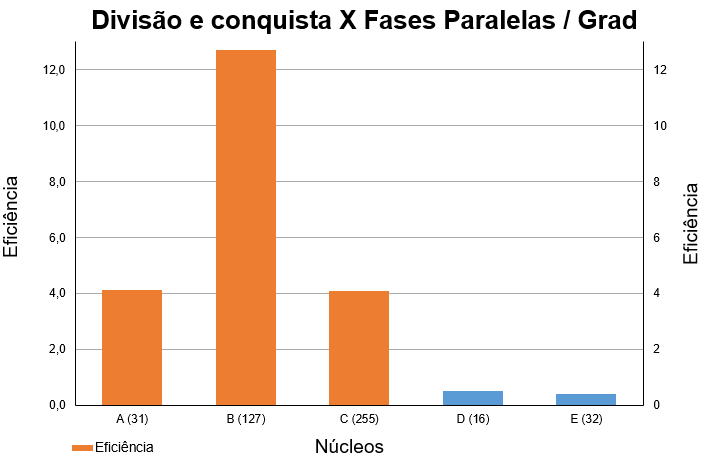
\includegraphics[width=9cm, height=4cm]{grafico.png}
            \vspace{-1.9em}
            \caption{Gráfico de Speed-up (A e C) e eficiência dos 3 casos}
            \vspace{-1.2em}
\end{figure}
\section{Observações Finais}


\end{multicols*}

\newpage

\lstinputlisting[language=C++]{tpp3.c}

\end{document}
